% ------------------------------------------------------------------------------
% Chapter 4
% ------------------------------------------------------------------------------
\chapter{Results} % enter the name of the chapter here
\label{cha:ch4_results} % enter the chapter label here (for cross referencing)

\section{Introduction}
\label{sec:Ch4 Introduction}
This chapter presents the results of the data analysis described in Chapter Three. The chapter follows the two-stage analytical strategy set out in Section~\ref{sec:Data Analysis}: it first reports the sample profile, data screening, descriptive statistics, reliability, common method bias, and preliminary Pearson correlations; it then reports the partial least squares structural equation model (PLS-SEM), covering the measurement model, discriminant validity, the choice of ROI specification, the structural model and hypothesis tests, effect sizes, the mediation test, control variable effects, predictive assessment, and robustness checks. The chapter closes with a summary table mapping each hypothesis to its outcome.

In this chapter, two conventions for reporting statistics will be used consistently. Firstly, all Likert-type items were assigned values, coded from 1 (Strongly Agree) to 5 (Strongly Disagree), where  \emph{lower} mean score indicates \emph{higher} levels of agreement, which is directed coding that differs from the more commonly used approach that recognizes higher scores as representative of higher agreement levels. Every mean reported below is interpreted with this direction in mind. Secondly, the PLS-SEM statistics reported in Sections~\ref{sec:Measurement Model}--\ref{sec:Robustness and Sensitivity Analysis} were computed using a Python-based implementation of the partial least squares algorithm rather than the SmartPLS software package; both implement the same underlying algorithm, and every statistic reported in this chapter, including the Dijkstra-Henseler consistency reliability coefficient (rho\textsubscript{A}), computed directly from the fitted model's outer weights and indicator correlation matrix using Dijkstra and Henseler's (2015) closed-form estimator \autocite{Dijkstra2015}, is reported alongside Cronbach's alpha and composite reliability (Dillon-Goldstein's rho) rather than in place of them.

\section{Data Screening and Sample Profile}
\label{sec:Data Screening and Sample Profile}
A total of 357 responses were submitted. Two respondents indicated that their team did not use an AI coding assistant and were excluded under the study's pre-specified eligibility criterion, leaving 355 eligible responses, consistent with the primary eligibility rule for this dataset. Among these 355 eligible responses, one respondent had a single missing value on a substantive item (a workflow-level ROI item); following the complete-case rule specified in Chapter Three, this respondent was excluded, yielding a final analytical sample of $N = 354$. This 354 arises from a missing-data exclusion applied after the primary eligibility rule, and not from any additional role-based exclusion. Table~\ref{tab:sample_flow} summarises this response flow.

\begin{table}[htbp]
	\centering
	\caption{Sample eligibility and participant flow}
	\label{tab:sample_flow}
	\begin{tabular}{lr}
		\hline
		\textbf{Stage} & \textbf{n} \\
		\hline
		Responses submitted & 357 \\
		Excluded: team does not use an AI coding assistant & $-2$ \\
		Eligible sample (primary rule) & 355 \\
		Excluded: incomplete response on a substantive item & $-1$ \\
		Final analytical sample & 354 \\
		\hline
	\end{tabular}
\end{table}

Table~\ref{tab:demographic_profile} summarises the demographic and usage profile of the final analytical sample. Respondents were predominantly software developers and senior developers, most commonly worked in teams of six to twenty engineers, most commonly had between two and ten years of professional development experience, and most commonly had used AI coding assistants for between one and two years.

\begin{table}[htbp]
	\centering
	\caption{Participant demographic and usage profile ($N = 354$)}
	\label{tab:demographic_profile}
	\resizebox{\linewidth}{!}{%
		\begin{tabular}{llrr}
			\hline
			\textbf{Characteristic} & \textbf{Category} & \textbf{n} & \textbf{Valid \%} \\
			\hline
			Role & Software Developer & 179 & 50.6 \\
			& Senior Developer & 92 & 26.0 \\
			& Technical Lead & 45 & 12.7 \\
			& Engineering Manager & 19 & 5.4 \\
			& Other roles (combined) & 19 & 5.4 \\
			\hline
			Team size & 6 -- 10 developers & 163 & 46.0 \\
			& 11 -- 20 developers & 86 & 24.3 \\
			& 1 -- 5 developers & 68 & 19.2 \\
			& More than 20 developers & 37 & 10.5 \\
			\hline
			Professional development experience & 2 -- 5 years & 154 & 43.5 \\
			& 6 -- 10 years & 133 & 37.6 \\
			& More than 10 years & 40 & 11.3 \\
			& Less than 2 years & 27 & 7.6 \\
			\hline
			AI coding assistant adoption duration & 1 -- 2 years & 197 & 55.6 \\
			& Less than 6 months & 76 & 21.5 \\
			& 6 -- 12 months & 73 & 20.6 \\
			& More than 2 years & 8 & 2.3 \\
			\hline
		\end{tabular}%
	}
\end{table}

No out-of-range values were found on any five-point item (all observed values fell between 1 and 5), and no evidence of exact duplicate submissions was identified from response timestamps.

\section{Descriptive Statistics}
\label{sec:Data Screening and Descriptive Statistics}
Table~\ref{tab:descriptives} reports descriptive statistics for each construct, computed as the mean of its constituent items. Every construct returned a low mean (all below 1.35 on the 1-to-5 scale) with pronounced positive skew and, in most cases, high kurtosis, indicating that the large majority of respondents selected ``Strongly Agree'' or ``Agree'' on almost every item, regardless of which construct was being measured. This pattern, a marked ceiling effect concentrated at the ``Strongly Agree'' end of the scale, is examined further in the common method bias assessment (Section~\ref{sec:Common Method Bias}) and tested directly in a dedicated sensitivity analysis (Section~\ref{sec:Robustness and Sensitivity Analysis}), which re-estimates the structural model after excluding the 247 of 354 respondents (69.8\%) who selected the most positive response option on every single substantive item.

\begin{table}[htbp]
	\centering
	\caption{Construct-level descriptive statistics ($N = 354$; scale 1 = Strongly Agree to 5 = Strongly Disagree)}
	\label{tab:descriptives}
	\resizebox{\linewidth}{!}{%
		\begin{tabular}{lrrrrrr}
			\hline
			\textbf{Construct} & \textbf{Mean} & \textbf{SD} & \textbf{Min} & \textbf{Max} & \textbf{Skewness} & \textbf{Kurtosis} \\
			\hline
			AI Leadership and Governance Support & 1.151 & 0.358 & 1.00 & 3.00 & 2.523 & 6.160 \\
			Organisational Culture & 1.139 & 0.338 & 1.00 & 3.00 & 2.456 & 5.413 \\
			Assimilation Quality & 1.254 & 0.487 & 1.00 & 4.00 & 2.151 & 5.558 \\
			ROI Overall (15 items) & 1.295 & 0.625 & 1.00 & 5.00 & 2.769 & 9.135 \\
			ROI Task-level (E1) & 1.271 & 0.604 & 1.00 & 5.00 & 3.199 & 13.230 \\
			ROI Workflow-level (E2) & 1.302 & 0.665 & 1.00 & 5.00 & 2.986 & 10.889 \\
			ROI Firm-level (E3) & 1.310 & 0.651 & 1.00 & 5.00 & 2.739 & 9.183 \\
			Organisational Readiness & 1.297 & 0.607 & 1.00 & 4.167 & 2.437 & 6.245 \\
			\hline
		\end{tabular}%
	}
\end{table}

\section{Reliability}
\label{sec:Reliability and Convergent Validity}
Table~\ref{tab:reliability} reports Cronbach's alpha and the range of corrected item-total correlations for each construct, computed separately for AI leadership and governance support, organisational culture, assimilation quality, organisational readiness, the 15-item ROI scale as a whole, and each of the three ROI dimensions. Every construct exceeded the conventional acceptability threshold of .70, and every corrected item-total correlation exceeded the conventional review threshold of .30 by a wide margin. Several constructs exceeded an alpha of .95, which, following the decision rule in Chapter Three, was inspected further rather than treated as automatically indicative of poor measurement; the inter-item correlations underlying these very high alphas are consistent with the extensive item redundancy already visible in the ROI sub-scale intercorrelations, and are discussed alongside the common method bias assessment below.

\begin{table}[htbp]
	\centering
	\caption{Reliability results ($N = 354$)}
	\label{tab:reliability}
	\resizebox{\linewidth}{!}{%
		\begin{tabular}{lrrr}
			\hline
			\textbf{Construct} & \textbf{Items} & \textbf{Cronbach's alpha} & \textbf{Item-total $r$ range} \\
			\hline
			AI Leadership and Governance Support & 4 & .878 & .652 -- .794 \\
			Organisational Culture & 7 & .963 & .821 -- .910 \\
			Assimilation Quality & 8 & .960 & .837 -- .875 \\
			ROI Overall (15 items) & 15 & .990 & .902 -- .958 \\
			ROI Task-level (E1) & 5 & .980 & .916 -- .958 \\
			ROI Workflow-level (E2) & 4 & .976 & .929 -- .954 \\
			ROI Firm-level (E3) & 6 & .977 & .908 -- .946 \\
			Organisational Readiness & 6 & .974 & .894 -- .934 \\
			\hline
		\end{tabular}%
	}
\end{table}

No item's removal was considered on reliability grounds alone: every corrected item-total correlation exceeded .65, well above the .30 review threshold, so there was no diagnostic basis for treating any single item as a weak indicator at this stage. The measurement model in Section~\ref{sec:Measurement Model} provides a second, independent check on indicator quality through outer loadings.

\section{Common Method Bias}
\label{sec:Common Method Bias}
Because all constructs were measured through self-report from the same respondents at the same point in time, common method bias was assessed using two independent procedures, following recommended practice for single-source survey designs \autocite{Hair2019}.

First, Harman's single-factor test was conducted: an unrotated principal component analysis was run on all 40 substantive items (AI leadership and governance support, organisational culture, assimilation quality, the 15 ROI items, and organisational readiness). Four components had an eigenvalue above 1, but the first unrotated factor alone accounted for 65.4\% of the total variance, well above the conventional 50\% threshold used to flag common method bias as a material concern.

Second, a full-collinearity variance inflation factor (VIF) test was conducted \autocite{Kock2015}, in which every construct (including the three single-indicator controls) was regressed on every other construct in the model, with a full-collinearity VIF at or below 3.3 taken as evidence that common method bias is unlikely to be a serious problem. Figure~\ref{fig:cmb_harman} summarises the Harman's single-factor result graphically, and Table~\ref{tab:full_collinearity_vif} reports the full-collinearity VIF results.

\begin{figure}[htbp]
	\centering
	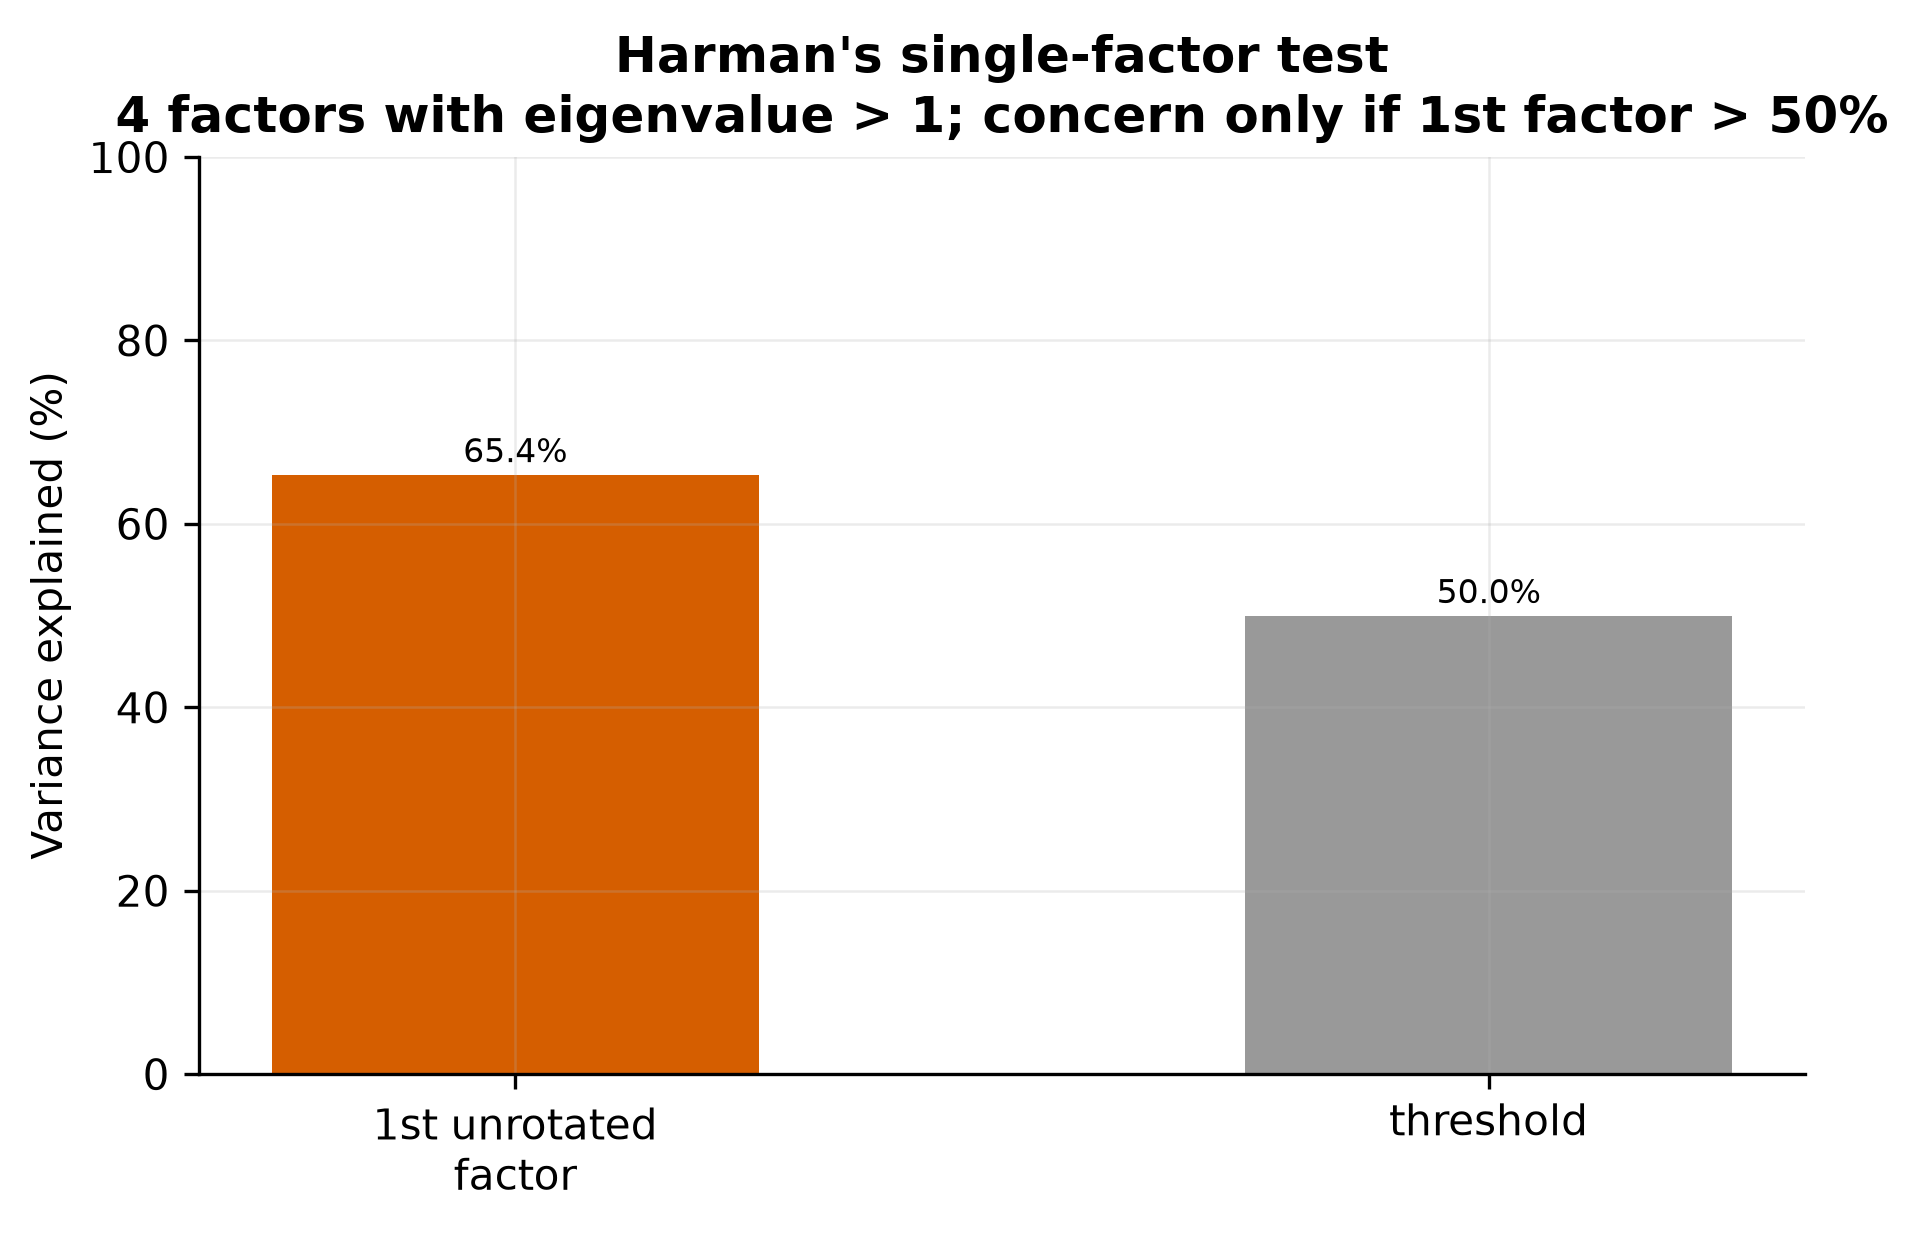
\includegraphics[width=0.75\linewidth]{Images/28_cmb_harman.png}
	\caption{Common method bias check: variance explained by successive unrotated principal components, with the first-factor threshold used by Harman's single-factor test.}
	\label{fig:cmb_harman}
\end{figure}

\begin{table}[htbp]
	\centering
	\caption{Full-collinearity VIF test for common method bias (Kock, 2015)}
	\label{tab:full_collinearity_vif}
	\begin{tabular}{lr}
		\hline
		\textbf{Construct} & \textbf{Full-collinearity VIF} \\
		\hline
		ROI & 5.422 \\
		Assimilation Quality & 5.035 \\
		Organisational Readiness & 4.846 \\
		Organisational Culture & 4.041 \\
		AI Leadership and Governance Support & 3.218 \\
		Developer Experience & 1.580 \\
		Team Size & 1.451 \\
		Adoption Duration & 1.115 \\
		\hline
	\end{tabular}
\end{table}

Five of the eight constructs, ROI, assimilation quality, organisational readiness, organisational culture, and AI leadership and governance support, exceeded the 3.3 threshold, with ROI itself reaching 5.422. Because this test is unrelated to the ceiling-effect analysis and does not simply restate the single-factor result, its agreement with Harman's test is informative rather than redundant: two different procedures, one based on the covariance structure of a single unrotated component and the other based on inter-construct collinearity, converge on the same conclusion. Common method bias is therefore treated as a genuine, and now doubly corroborated, concern for this dataset, to be borne in mind throughout the interpretation of the results that follow; it is revisited in the discussion of the structural model's discriminant validity (Section~\ref{sec:Discriminant validity}) and in Chapter Five.

\section{Preliminary Correlations}
\label{sec:Preliminary Correlations}
Following the reliability assessment, provisional mean scores were computed for each construct, and Pearson correlations were computed among them as a preliminary, descriptive step (Section~\ref{sec:Data Analysis}); these correlations are not the confirmatory test of the study's hypotheses, which is reported in Section~\ref{sec:Structural Model and Hypothesis Testing}. Table~\ref{tab:prelim_corr} reports the resulting correlation matrix; all coefficients were statistically significant at $p < .001$.

\begin{table}[htbp]
	\centering
	\caption{Preliminary Pearson correlations among provisional construct mean scores ($N = 354$, all $p < .001$)}
	\label{tab:prelim_corr}
	\resizebox{\linewidth}{!}{%
		\begin{tabular}{lrrrrrrrr}
			\hline
			& \textbf{Leadership} & \textbf{Culture} & \textbf{Assim.} & \textbf{ROI} & \textbf{E1} & \textbf{E2} & \textbf{E3} & \textbf{Readiness} \\
			\hline
			Leadership & 1.000 & & & & & & & \\
			Culture & 0.812 & 1.000 & & & & & & \\
			Assimilation Quality & 0.605 & 0.693 & 1.000 & & & & & \\
			ROI Overall & 0.446 & 0.531 & 0.830 & 1.000 & & & & \\
			ROI Task-level (E1) & 0.427 & 0.522 & 0.818 & 0.974 & 1.000 & & & \\
			ROI Workflow-level (E2) & 0.428 & 0.499 & 0.809 & 0.987 & 0.968 & 1.000 & & \\
			ROI Firm-level (E3) & 0.449 & 0.532 & 0.810 & 0.975 & 0.906 & 0.940 & 1.000 & \\
			Organisational Readiness & 0.440 & 0.505 & 0.812 & 0.877 & 0.851 & 0.855 & 0.866 & 1.000 \\
			\hline
		\end{tabular}%
	}
\end{table}

Two features of this matrix are notable in light of the discriminant validity results reported in Section~\ref{sec:Discriminant validity}. First, AI leadership and governance support and organisational culture were very highly correlated ($r = .812$). Second, the three ROI dimensions were correlated with one another at $r = .906$ to $.987$, and each was correlated with organisational readiness at $r = .851$ to $.866$, correlations high enough to raise a diagnostic concern about construct overlap (the manual's diagnostic trigger of $r > .80$), which is examined formally below.

\section{Measurement Model}
\label{sec:Measurement Model}
A reflective measurement model was estimated for AI leadership and governance support, organisational culture, assimilation quality, ROI, and organisational readiness, together with the three single-indicator control variables (team size, developer experience, and adoption duration). Table~\ref{tab:measurement_model} reports the range of outer loadings for each construct, together with Cronbach's alpha, composite reliability (Dillon-Goldstein's rho), and average variance extracted (AVE).

\begin{table}[htbp]
	\centering
	\caption{Measurement model: outer loadings, reliability, and convergent validity}
	\label{tab:measurement_model}
	\resizebox{\linewidth}{!}{%
		\begin{tabular}{lrrrrr}
			\hline
			\textbf{Construct} & \textbf{Loading range} & \textbf{Alpha} & \textbf{rho\textsubscript{A}} & \textbf{CR (Dillon-Goldstein)} & \textbf{AVE} \\
			\hline
			AI Leadership and Governance Support & .840 -- .879 & .885 & .896 & .921 & .740 \\
			Organisational Culture & .872 -- .932 & .964 & .970 & .970 & .822 \\
			Assimilation Quality & .859 -- .911 & .963 & .968 & .969 & .792 \\
			ROI Overall (15 items) & .909 -- .962 & .990 & .992 & .991 & .880 \\
			Organisational Readiness & .923 -- .955 & .975 & .976 & .980 & .889 \\
			\hline
		\end{tabular}%
	}
\end{table}

Every indicator loaded above .708 on its intended construct, the strong-loading threshold set out in Chapter Three, so no indicator was removed from the measurement model. Composite reliability exceeded .90 for every reflective construct (a level the review threshold in Chapter Three treats as a potential redundancy flag for constructs already showing an alpha above .95), and AVE exceeded .50 for every construct by a considerable margin (ranging from .740 for AI leadership and governance support to .889 for organisational readiness), indicating that each construct's indicators captured well over half of that construct's variance. rho\textsubscript{A} was computed directly from the fitted model's outer weights using Dijkstra and Henseler's (2015) closed-form estimator \autocite{Dijkstra2015} and fell, as expected, between Cronbach's alpha and composite reliability for every construct except ROI, whose three internal-consistency statistics (alpha $=.990$, rho\textsubscript{A}$=.992$, CR$=.991$) were effectively indistinguishable from one another to three decimal places, reflecting the extremely homogeneous, near-unidimensional response pattern already flagged for the 15-item ROI scale in Section~\ref{sec:Data Screening and Descriptive Statistics} and revisited in the common method bias assessment below. All three internal-consistency statistics, and rho\textsubscript{A} in particular, point to the same conclusion of strong, and for several constructs arguably redundant, internal consistency.

\section{Discriminant Validity}
\label{sec:Discriminant validity}
Discriminant validity was assessed using three procedures: the heterotrait-monotrait ratio of correlations (HTMT), with a bootstrapped confidence interval for every ratio; the Fornell-Larcker criterion; and an inspection of item cross-loadings. Table~\ref{tab:htmt} reports the HTMT matrix for the baseline model (with ROI represented as a single overall construct), together with the 95\% bootstrap confidence interval (percentile method, 2,000 resamples, fixed seed) for each ratio.

\begin{table}[htbp]
	\centering
	\caption{HTMT discriminant validity matrix, with bootstrap 95\% confidence intervals}
	\label{tab:htmt}
	\resizebox{\linewidth}{!}{%
		\begin{tabular}{llrrr}
			\hline
			\textbf{Pair} & & \textbf{HTMT} & \textbf{95\% CI lower} & \textbf{95\% CI upper} \\
			\hline
			Leadership & Culture & .881 & .776 & .967 \\
			Leadership & Assimilation Quality & .670 & .544 & .783 \\
			Leadership & ROI & .477 & .350 & .636 \\
			Leadership & Organisational Readiness & .475 & .347 & .616 \\
			Culture & Assimilation Quality & .728 & .637 & .808 \\
			Culture & ROI & .543 & .427 & .676 \\
			Culture & Organisational Readiness & .521 & .394 & .657 \\
			Assimilation Quality & ROI & .851 & .799 & .904 \\
			Assimilation Quality & Organisational Readiness & .841 & .756 & .916 \\
			ROI & Organisational Readiness & .895 & .816 & .951 \\
			\hline
		\end{tabular}%
	}
\end{table}

Most HTMT point estimates fell below the strong-evidence threshold of .85. Three values fell in the borderline range of .85 to .90: AI leadership and governance support versus organisational culture (HTMT $= .881$), assimilation quality versus ROI (HTMT $= .851$), and ROI versus organisational readiness (HTMT $= .895$); assimilation quality versus organisational readiness was just below this band (HTMT $= .841$). The bootstrap confidence intervals sharpen this picture in the way Hair et al. (2019) recommend \autocite{Hair2019}: every interval's upper bound remained below 1, so no pair of constructs can be said to be statistically indistinguishable from a single construct. However, for exactly these four pairs, leadership-culture, assimilation-ROI, assimilation-readiness, and ROI-readiness, the confidence interval's upper bound exceeded .90 (reaching as high as .967 for leadership-culture and .951 for ROI-readiness), meaning discriminant validity between these four pairs cannot be established with confidence even at the more lenient .90 threshold, only that the two constructs in each pair are not perfectly identical. For every other pair, the upper bound remained comfortably below .90, giving strong inferential, and not merely point-estimate, evidence of discriminant validity. Following the reporting template in Chapter Three, these results were not treated as invalidating the measurement model outright, but as identifying four specific pairs of constructs whose independent, discriminant contribution should be interpreted cautiously; this caution is reflected in the structural model results in Section~\ref{sec:Structural Model and Hypothesis Testing}, where AI leadership and governance support's direct effects are estimated with less precision than would be expected from its preliminary correlation with ROI, plausibly because a substantial part of what the leadership items measure overlaps with what the culture items measure, and in the discussion of organisational readiness's dominant effect in Chapter Five, which should be read alongside its borderline discriminant validity from both assimilation quality and ROI.

As a complement to HTMT, Table~\ref{tab:discriminant_fl} reports the Fornell-Larcker criterion: the square root of each construct's AVE on the diagonal, compared against its correlation with every other construct off the diagonal.

\begin{table}[htbp]
	\centering
	\caption{Fornell-Larcker discriminant validity matrix (diagonal = $\sqrt{\mathrm{AVE}}$)}
	\label{tab:discriminant_fl}
	\resizebox{\linewidth}{!}{%
		\begin{tabular}{lrrrrr}
			\hline
			& \textbf{Leadership} & \textbf{Culture} & \textbf{Assim.} & \textbf{ROI} & \textbf{Readiness} \\
			\hline
			Leadership & \textbf{.860} & & & & \\
			Culture & .817 & \textbf{.907} & & & \\
			Assimilation Quality & .608 & .689 & \textbf{.890} & & \\
			ROI & .453 & .533 & .830 & \textbf{.938} & \\
			Organisational Readiness & .445 & .505 & .810 & .877 & \textbf{.943} \\
			\hline
		\end{tabular}%
	}
\end{table}

By the Fornell-Larcker criterion, every construct's $\sqrt{\mathrm{AVE}}$ exceeded its correlation with every other construct, formally satisfying the criterion for all five constructs, including the four pairs flagged as borderline by the HTMT confidence intervals above (for example, ROI's $\sqrt{\mathrm{AVE}}$ of .938 exceeds its .877 correlation with organisational readiness, though only by .061). This divergence between HTMT and Fornell-Larcker is itself a well-documented property of the two criteria rather than a contradiction in the data: \textcite{Henseler2015} show that Fornell-Larcker is a comparatively conservative test that under-detects discriminant validity problems that HTMT is specifically designed to catch, which is why HTMT, not Fornell-Larcker, is treated as the primary discriminant validity criterion in this study, consistent with Chapter Three; the Fornell-Larcker result is reported as supplementary, corroborating evidence at the level the construct-correlation matrix can provide, not as evidence overriding the HTMT-based caution above.

Finally, cross-loadings were inspected for every one of the 40 substantive items: an item's correlation with its own (home) construct's score was compared against its correlation with every other construct's score. All 40 items loaded most strongly on their intended construct, so no item was flagged for possible mis-specification on this third discriminant validity criterion. The margin between an item's home-construct and next-highest cross-construct correlation varied considerably, from as little as .053 for one organisational readiness item up to .227 for one leadership item; the narrowest margins were concentrated among the organisational readiness and firm-level ROI items, consistent with the borderline HTMT evidence for the assimilation-ROI and ROI-readiness pairs reported above, while no item crossed over to load more strongly on a different construct than its own.

\subsection{ROI Specification: Overall Versus Dimensional}
\label{sec:ROI Specification}
Because the theoretical framework identifies ROI at three levels, task, workflow, and firm, a dimensional measurement model was also estimated, with task-level ROI (E1), workflow-level ROI (E2), and firm-level ROI (E3) specified as three separate reflective constructs. Table~\ref{tab:htmt_dimensional} reports the resulting HTMT values among the three dimensions and the remaining constructs.

\begin{table}[htbp]
	\centering
	\caption{HTMT discriminant validity: dimensional ROI specification}
	\label{tab:htmt_dimensional}
	\resizebox{\linewidth}{!}{%
		\begin{tabular}{lrrr}
			\hline
			& \textbf{Task ROI (E1)} & \textbf{Workflow ROI (E2)} & \textbf{Firm ROI (E3)} \\
			\hline
			Task ROI (E1) & -- & & \\
			Workflow ROI (E2) & .988 & -- & \\
			Firm ROI (E3) & .924 & .962 & -- \\
			\hline
		\end{tabular}%
	}
\end{table}

All three pairwise HTMT values among the ROI dimensions substantially exceeded the .90 threshold, indicating that task-, workflow-, and firm-level ROI could not be empirically distinguished from one another in this sample. The dimensional structural model (Table~\ref{tab:dimensional_paths}) told materially the same substantive story as the overall model, with very similar predictor patterns and only slightly lower explained variance for each dimension (task-level $R^2 = .780$; workflow-level $R^2 = .777$; firm-level $R^2 = .786$) than for the overall 15-item construct ($R^2 = .816$, Section~\ref{sec:Explanatory Power}). On the combined weight of this measurement evidence, the theoretical argument that a single underlying perceived-ROI construct is being expressed through three related item sets, and the requirement in Chapter Three that this choice be justified by evidence rather than by whichever specification yields more significant paths, the overall 15-item ROI construct was selected as the final specification reported in the structural model below. The dimensional model is retained here as supporting evidence for that decision and is not used for hypothesis testing.

\begin{table}[htbp]
	\centering
	\caption{Structural paths under the dimensional ROI specification (bootstrap, 2,000 resamples)}
	\label{tab:dimensional_paths}
	\resizebox{\linewidth}{!}{%
		\begin{tabular}{lrrrrr}
			\hline
			\textbf{Path} & \textbf{Task ROI $\beta$} & \textbf{Workflow ROI $\beta$} & \textbf{Firm ROI $\beta$} \\
			\hline
			Assimilation Quality $\rightarrow$ ROI dimension & .388$^{**}$ & .371$^{**}$ & .297$^{*}$ \\
			AI Leadership and Governance Support $\rightarrow$ ROI dimension & $-$.101 & $-$.046 & $-$.043 \\
			Organisational Culture $\rightarrow$ ROI dimension & .076 & .011 & .074 \\
			Organisational Readiness $\rightarrow$ ROI dimension & .544$^{***}$ & .568$^{***}$ & .606$^{***}$ \\
			Team Size $\rightarrow$ ROI dimension & .055 & .046 & .003 \\
			Developer Experience $\rightarrow$ ROI dimension & .062 & .076 & .056 \\
			Adoption Duration $\rightarrow$ ROI dimension & $-$.028 & $-$.028 & $-$.035 \\
			\hline
			\multicolumn{4}{l}{\footnotesize $^{*}p<.05$, $^{**}p<.01$, $^{***}p<.001$; coefficients are unstandardised PLS path coefficients on standardised indicators.}
		\end{tabular}%
	}
\end{table}

\section{Structural Model and Hypothesis Testing}
\label{sec:Structural Model and Hypothesis Testing}

\subsection{Collinearity}
\label{sec:Collinearity}
Inner variance inflation factors (VIF) were inspected before interpreting the structural path coefficients. Table~\ref{tab:vif} reports the results. All VIF values fell below the serious-collinearity threshold of 5; organisational culture and assimilation quality fell in the 3-to-5 range that Chapter Three treats as warranting cautious interpretation of individual coefficients, consistent with the high correlation between culture and leadership already noted.

\begin{table}[htbp]
	\centering
	\caption{Inner VIF for predictors of ROI, and of Assimilation Quality}
	\label{tab:vif}
	\resizebox{\linewidth}{!}{%
		\begin{tabular}{lr}
			\hline
			\textbf{Predictor of ROI} & \textbf{VIF} \\
			\hline
			Assimilation Quality & 4.474 \\
			Organisational Culture & 4.007 \\
			AI Leadership and Governance Support & 3.125 \\
			Organisational Readiness & 3.018 \\
			Developer Experience & 1.558 \\
			Team Size & 1.445 \\
			Adoption Duration & 1.115 \\
			\hline
			\textbf{Predictor of Assimilation Quality} & \textbf{VIF} \\
			\hline
			Organisational Culture & 2.940 \\
			AI Leadership and Governance Support & 2.940 \\
			\hline
		\end{tabular}%
	}
\end{table}

\subsection{Direct Effects and Hypothesis Testing}
\label{sec:Direct Effects}
Structural path coefficients were estimated with bootstrapping (2,000 resamples, percentile method, two-tailed test). Table~\ref{tab:structural_paths} reports the unstandardised path coefficient ($\beta$), bootstrap standard error, $t$-statistic, approximate $p$-value, and 95\% confidence interval for every path in the baseline (overall ROI) structural model.

\begin{table}[htbp]
	\centering
	\caption{Structural path coefficients (bootstrap, 2,000 resamples)}
	\label{tab:structural_paths}
	\resizebox{\linewidth}{!}{%
		\begin{tabular}{lrrrrr}
			\hline
			\textbf{Path} & \textbf{$\beta$} & \textbf{SE} & \textbf{$t$} & \textbf{$p$} & \textbf{95\% CI} \\
			\hline
			Organisational Culture $\rightarrow$ Assimilation Quality & .579 & .125 & 4.64 & $<.001$ & [.348, .820] \\
			AI Leadership and Governance Support $\rightarrow$ Assimilation Quality & .135 & .138 & 0.98 & .328 & [$-$.142, .385] \\
			Assimilation Quality $\rightarrow$ ROI & .356 & .147 & 2.43 & .015 & [.063, .624] \\
			Organisational Culture $\rightarrow$ ROI (direct) & .057 & .068 & 0.83 & .407 & [$-$.090, .194] \\
			AI Leadership and Governance Support $\rightarrow$ ROI (direct) & $-$.063 & .054 & $-$1.16 & .247 & [$-$.158, .051] \\
			Organisational Readiness $\rightarrow$ ROI & .588 & .135 & 4.35 & $<.001$ & [.344, .871] \\
			Team Size $\rightarrow$ ROI & .031 & .039 & 0.80 & .422 & [$-$.068, .074] \\
			Developer Experience $\rightarrow$ ROI & .065 & .047 & 1.36 & .173 & [$-$.076, .128] \\
			Adoption Duration $\rightarrow$ ROI & $-$.032 & .025 & $-$1.29 & .196 & [$-$.078, .019] \\
			\hline
		\end{tabular}%
	}
\end{table}

Three results bear directly on H1 to H3. First, organisational culture had a strong, statistically significant effect on assimilation quality, but its \emph{direct} effect on ROI, once assimilation quality and the four controls were included in the same model, was small and not statistically significant. Second, AI leadership and governance support's effect on assimilation quality, and its direct effect on ROI, were both small and not statistically significant. Third, assimilation quality had a statistically significant, positive direct effect on ROI. Because H1 and H2 concern the \emph{overall} association between each predictor and ROI, they were evaluated using the total effect (direct plus indirect via assimilation quality, Section~\ref{sec:Mediation Analysis Results}) rather than the direct effect alone; on that basis, H1 was supported (organisational culture's total effect on ROI was positive and, as shown below, its indirect component was statistically significant), while H2 was not supported (AI leadership and governance support's indirect effect was not statistically significant, and its direct effect was likewise not statistically significant, so no component of its total effect met the threshold for statistical support). This is a materially different conclusion from the preliminary Pearson correlation reported in Section~\ref{sec:Preliminary Correlations}, where both culture and leadership were significantly correlated with ROI; the structural model shows that, once the shared variance between culture and leadership and the four control variables are accounted for simultaneously, leadership's association with ROI does not hold up, illustrating directly why Chapter Three treats the preliminary correlations as screening evidence rather than as the confirmatory hypothesis test. H3 was supported: assimilation quality had a statistically significant, positive effect on ROI net of organisational culture, AI leadership and governance support, and all four controls.

Figure~\ref{fig:path_model} presents the estimated structural model in diagrammatic form, with each path's coefficient, significance, and the $R^2$ of each endogenous construct, to summarise the pattern described above at a glance.

\begin{figure}[htbp]
	\centering
	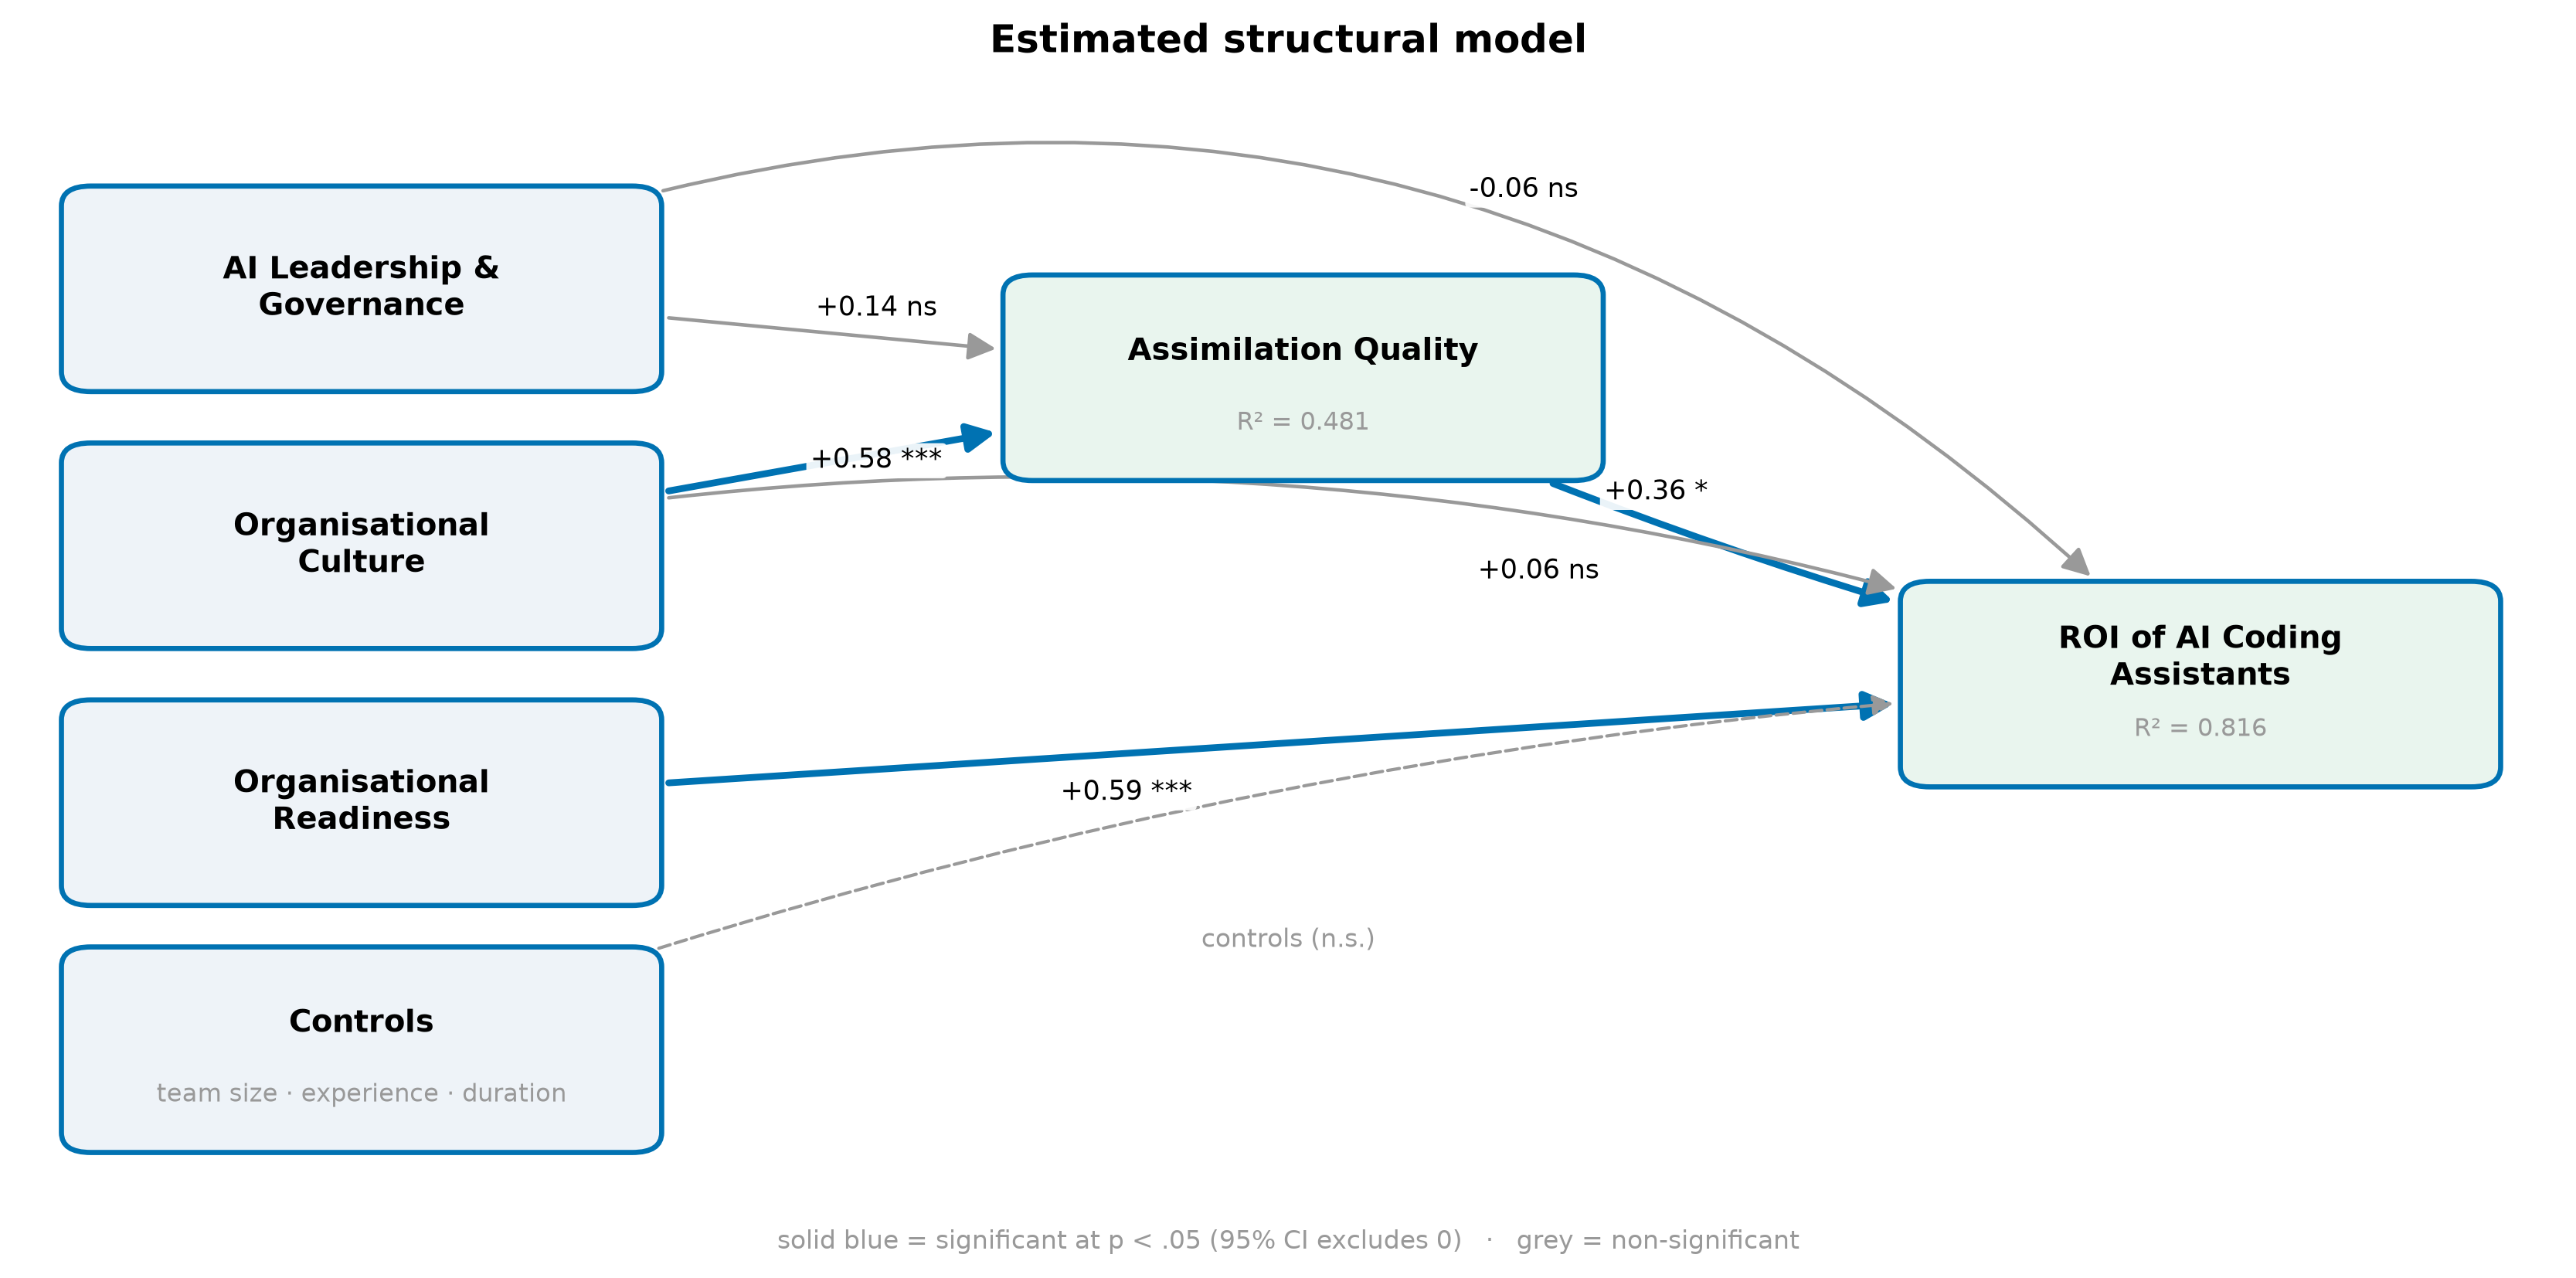
\includegraphics[width=\linewidth]{Images/17_path_model_diagram.png}
	\caption{Estimated structural model. Solid blue paths are statistically significant at $p<.05$ (95\% bootstrap confidence interval excludes zero); grey paths are not statistically significant.}
	\label{fig:path_model}
\end{figure}

\subsection{Explanatory Power and Effect Sizes}
\label{sec:Explanatory Power}
Table~\ref{tab:r2_f2} reports $R^2$, adjusted $R^2$, and $f^2$ effect sizes for the endogenous constructs.

\begin{table}[htbp]
	\centering
	\caption{$R^2$, adjusted $R^2$, and $f^2$ effect sizes}
	\label{tab:r2_f2}
	\resizebox{\linewidth}{!}{%
		\begin{tabular}{lrr}
			\hline
			\textbf{Endogenous construct} & \textbf{$R^2$} & \textbf{Adjusted $R^2$} \\
			\hline
			Assimilation Quality & .481 & .478 \\
			ROI & .816 & .812 \\
			\hline
			\textbf{Predictor of ROI} & \textbf{$f^2$} & \\
			\hline
			Organisational Readiness & .626 & (large) \\
			Assimilation Quality & .157 & (small-to-medium) \\
			Developer Experience & .015 & (negligible) \\
			Adoption Duration & .005 & (negligible) \\
			AI Leadership and Governance Support & .007 & (negligible) \\
			Team Size & .004 & (negligible) \\
			Organisational Culture & .004 & (negligible) \\
			\hline
			\textbf{Predictor of Assimilation Quality} & \textbf{$f^2$} & \\
			\hline
			Organisational Culture & .211 & (medium) \\
			AI Leadership and Governance Support & .011 & (negligible) \\
			\hline
		\end{tabular}%
	}
\end{table}

The structural model explained 48.1\% of the variance in assimilation quality and 81.6\% of the variance in ROI. The effect-size pattern reinforces the path-coefficient results: organisational readiness made, by a considerable margin, the largest individual contribution to explained variance in ROI ($f^2 = .626$, a large effect), ahead of assimilation quality ($f^2 = .157$), while organisational culture, AI leadership and governance support, and the three demographic controls each made a negligible direct contribution to ROI once the other predictors were held constant. For assimilation quality, organisational culture made a medium contribution ($f^2 = .211$) and AI leadership and governance support a negligible one ($f^2 = .011$), mirroring the path-coefficient pattern in Table~\ref{tab:structural_paths}.

\section{Mediation Analysis}
\label{sec:Mediation Analysis Results}
H4 proposed that assimilation quality mediates the relationship between (a) organisational culture and (b) AI leadership and governance support, and ROI. The specific indirect effect for each path was estimated as the product of the relevant path to assimilation quality and the path from assimilation quality to ROI, with its own bootstrapped 95\% confidence interval (2,000 resamples). Table~\ref{tab:mediation} reports the results, together with the direct effect for the same predictor and the resulting mediation classification, following the classification scheme in Chapter Three.

\begin{table}[htbp]
	\centering
	\caption{Specific indirect effects and mediation classification}
	\label{tab:mediation}
	\resizebox{\linewidth}{!}{%
		\begin{tabular}{lrrrrl}
			\hline
			\textbf{Path} & \textbf{Indirect $\beta$} & \textbf{95\% CI} & \textbf{Direct $\beta$} & \textbf{95\% CI} & \textbf{Classification} \\
			\hline
			Culture $\rightarrow$ Assimilation $\rightarrow$ ROI & .206$^{*}$ & [.025, .409] & .057 (ns) & [$-$.090, .194] & Indirect-only mediation \\
			Leadership $\rightarrow$ Assimilation $\rightarrow$ ROI & .048 (ns) & [$-$.057, .171] & $-$.063 (ns) & [$-$.158, .051] & No support for mediation \\
			\hline
			\multicolumn{6}{l}{\footnotesize $^{*}p<.05$; ns = not statistically significant (95\% CI includes zero).}
		\end{tabular}%
	}
\end{table}

For the organisational culture path, the indirect effect through assimilation quality was statistically significant (95\% CI excluded zero) while the direct effect was not, which the classification scheme in Chapter Three identifies as indirect-only mediation: culture's association with ROI in this sample operated through assimilation quality rather than through any additional direct channel. For the AI leadership and governance support path, neither the indirect effect nor the direct effect was statistically significant, so H4 was not supported for this path; assimilation quality cannot be said to mediate a relationship between leadership and ROI that was not itself established at either the direct or the indirect level. H4 was therefore partially supported: supported for the organisational culture pathway (H4a) and not supported for the AI leadership and governance support pathway (H4b).

\section{Control Variable Effects}
\label{sec:Control Variable Effects}
Table~\ref{tab:structural_paths} above reports the four control paths to ROI. Organisational readiness had, by a substantial margin, the strongest and most precisely estimated effect of any predictor in the model ($\beta = .588$, $p < .001$), exceeding even assimilation quality. None of team size, developer experience, or adoption duration had a statistically significant effect on ROI once the other predictors were included (all $p > .17$); developer experience showed the largest of the three coefficients, but its 95\% confidence interval still included zero. Because team size and developer experience are coded in ascending order (higher values indicating a larger team or more experience) while ROI retains the reversed Likert direction described in Section~\ref{sec:Ch4 Introduction}, a negative raw path coefficient corresponds to a positive association with perceived ROI and a positive raw coefficient corresponds to a negative association; applying this correction, adoption duration's coefficient ($\beta = -.032$, ns) corresponds to a small, statistically non-significant positive association between longer adoption duration and perceived ROI, and developer experience's coefficient ($\beta = .065$, ns) corresponds to a small, statistically non-significant negative association between greater developer experience and perceived ROI. None of these three associations reached statistical significance, and they are not interpreted further.

\section{Importance-Performance Map Analysis}
\label{sec:IPMA}
The path coefficients and effect sizes reported above establish which predictors matter statistically; they do not, on their own, indicate where managerial attention would be most productively directed, since a predictor's importance to ROI needs to be read alongside how well the organisation is already performing on that predictor. An importance-performance map analysis (IPMA) was therefore conducted for the four constructs with a hypothesised or control-variable path to ROI (organisational culture, AI leadership and governance support, assimilation quality, and organisational readiness), following standard PLS-SEM IPMA procedure \autocite{Hair2019}. Importance was operationalised as each construct's total standardised effect on ROI (direct effect plus, for culture and leadership, its indirect effect through assimilation quality); performance was operationalised by rescaling each construct's raw mean score (on the study's 1-to-5, Strongly-Agree-to-Strongly-Disagree scale) to a 0-to-100 index, where 100 represents the most positive possible score (a raw mean of 1, all ``Strongly Agree'') and 0 represents the least positive possible score (a raw mean of 5, all ``Strongly Disagree''). Table~\ref{tab:ipma} reports the results.

\begin{table}[htbp]
	\centering
	\caption{Importance-performance map analysis (target construct: ROI)}
	\label{tab:ipma}
	\resizebox{\linewidth}{!}{%
		\begin{tabular}{lrrr}
			\hline
			\textbf{Construct} & \textbf{Importance (total effect on ROI)} & \textbf{Mean (1--5 scale)} & \textbf{Performance (0--100)} \\
			\hline
			Organisational Readiness & .588 & 1.297 & 92.57 \\
			Assimilation Quality & .356 & 1.254 & 93.66 \\
			Organisational Culture & .262 & 1.139 & 96.52 \\
			AI Leadership and Governance Support & $-$.015 & 1.151 & 96.22 \\
			\hline
		\end{tabular}%
	}
\end{table}

Figure~\ref{fig:ipma} plots these results, with importance on the horizontal axis and performance on the vertical axis. Two features of the map are notable, and both reinforce conclusions reached elsewhere in this chapter through different evidence. First, organisational readiness combines the highest importance to ROI with the lowest performance score of the four constructs, placing it in the map's lower-right, ``priority for management action'' quadrant: it is simultaneously the construct ROI depends on most and the one on which respondents rated their organisations least positively, even though its absolute performance score (92.57) remains high in absolute terms given the ceiling effect that pervades this dataset. Second, AI leadership and governance support combines the lowest, and in fact a marginally negative, importance score with the second-highest performance score, placing it in the map's upper-left, ``high performance, low leverage'' quadrant; its near-zero importance reflects the total-effect calculation absorbing both its statistically non-significant direct effect on ROI and its statistically non-significant indirect effect through assimilation quality (Section~\ref{sec:Mediation Analysis Results}), so the negative sign should not be over-interpreted as evidence that leadership harms ROI, only that this study's structural model could not distinguish its total effect from zero. Because every item in this study is coded so that a lower raw score indicates stronger agreement, a positive importance value indicates that stronger agreement with a construct's items is associated with higher perceived ROI in the ordinary sense; this direction was confirmed for every construct's sign before interpreting the map. Read together with the effect-size results in Section~\ref{sec:Explanatory Power}, the IPMA provides a formal, quantified basis for the sequencing recommendation developed further in Chapter Five and Chapter Six: organisational readiness is both the most important and the least well-performing of the four constructs, making it the most defensible priority for managerial investment on this study's evidence.

\begin{figure}[htbp]
	\centering
	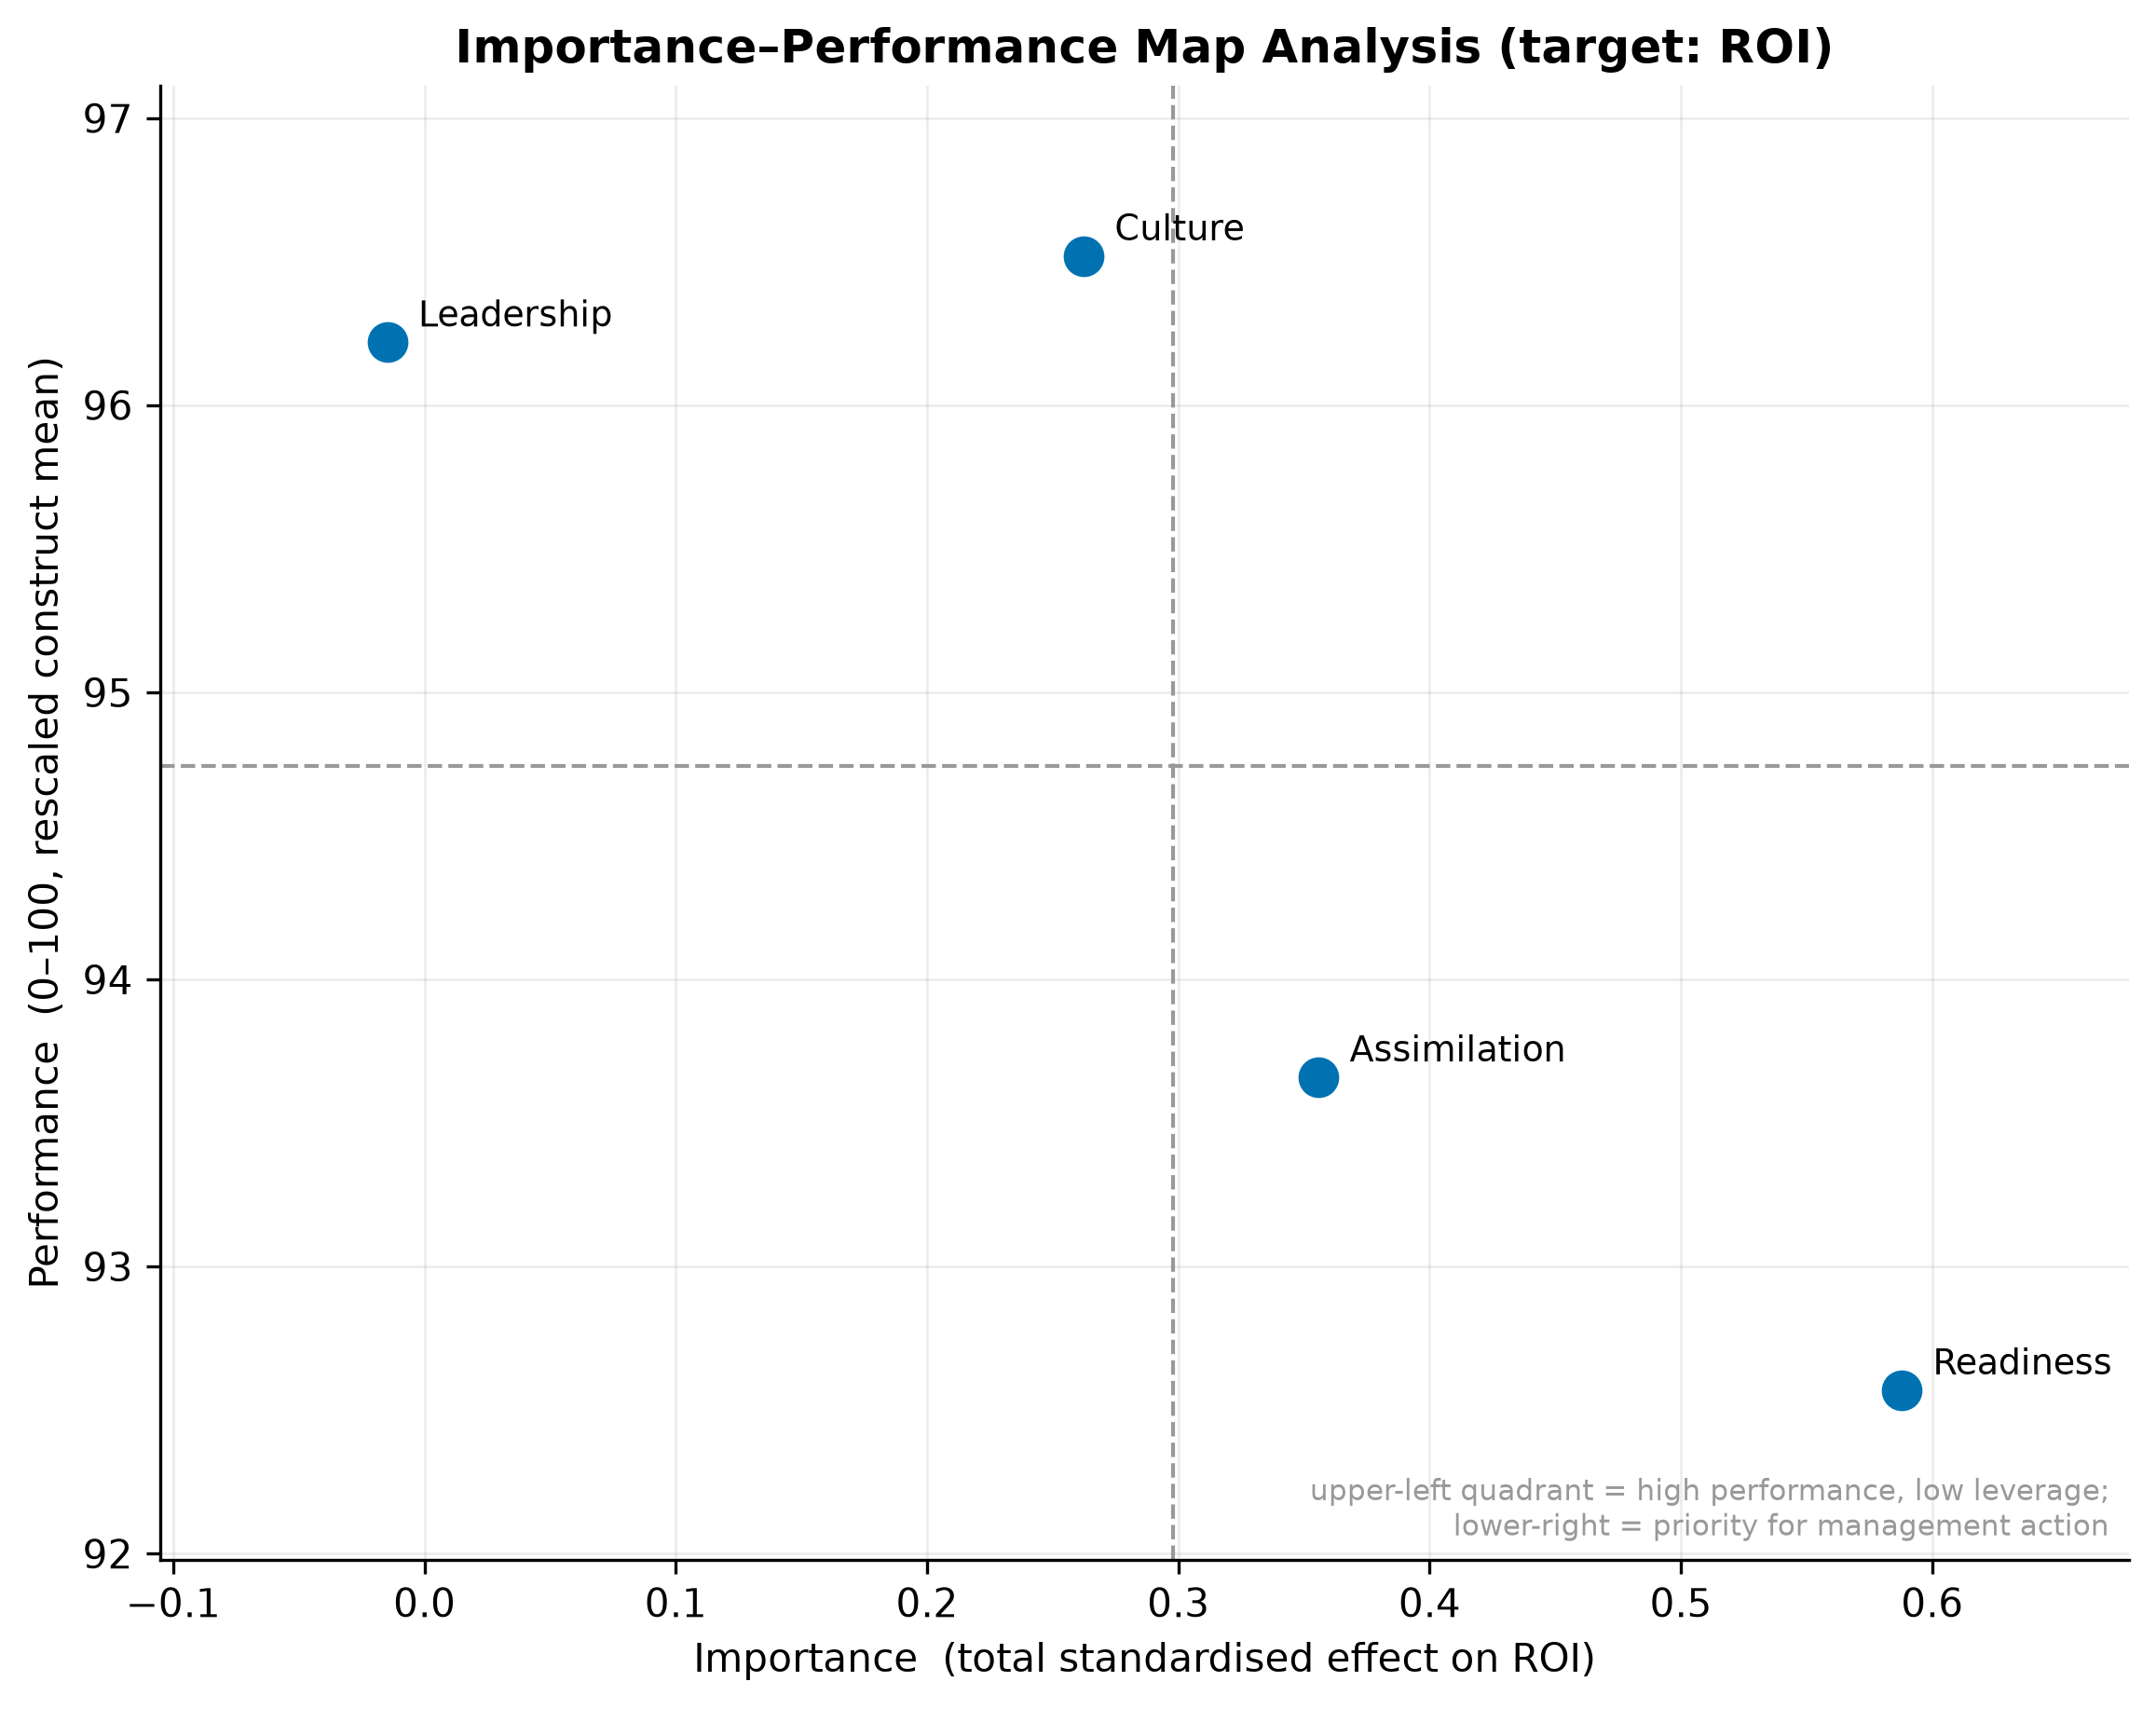
\includegraphics[width=0.8\linewidth]{Images/26_ipma.png}
	\caption{Importance-performance map for ROI. Lower-right quadrant (high importance, lower performance) indicates a priority for management action; upper-left (high performance, low importance) indicates a construct already performing well but with limited additional leverage over ROI.}
	\label{fig:ipma}
\end{figure}

\section{Supplementary Analysis: Individual Leadership Behaviours and ROI}
\label{sec:Leadership Behaviours Supplementary Analysis}
Research question 3 (Section~\ref{sec:Research questions}) asks which leadership behaviours most strongly affect ROI outcomes, a question about the relative contribution of the four specific behaviours, executive sponsorship, metric alignment, resource support, and governance clarity, rather than about the bundled four-item construct tested as a single predictor in H2. Because those four behaviours were measured with one item each (SL1 to SL4) and modelled as a single reflective construct in the structural model above, the structural test in Section~\ref{sec:Direct Effects} cannot, on its own, distinguish one behaviour's contribution from another's. To address RQ3 directly, this section reports the bivariate Pearson correlation between each individual leadership item and the overall ROI composite. This is a descriptive, item-level comparison rather than a further confirmatory structural test, and is reported as a supplementary analysis for this reason.

\begin{table}[htbp]
	\centering
	\caption{Individual leadership behaviours: correlation with ROI and PLS outer loading}
	\label{tab:leadership_items}
	\begin{tabular}{lrrr}
		\hline
		\textbf{Leadership behaviour (item)} & \textbf{$r$ with ROI} & \textbf{$p$} & \textbf{Outer loading} \\
		\hline
		Governance Clarity (SL4) & .431 & $<.001$ & .840 \\
		Executive Sponsorship (SL1) & .410 & $<.001$ & .853 \\
		Resource Support (SL3) & .360 & $<.001$ & .868 \\
		Metric Alignment (SL2) & .344 & $<.001$ & .879 \\
		\hline
	\end{tabular}
\end{table}

All four behaviours were significantly correlated with ROI at the item level ($p < .001$ in every case), and the differences between them were modest. Governance clarity, ensuring governance, risk, and quality concerns related to AI coding assistants are actively addressed, showed the strongest individual association with ROI ($r = .431$), followed closely by executive sponsorship ($r = .410$). Resource support ($r = .360$) and metric alignment ($r = .344$) showed somewhat weaker, though still significant, associations. This ordering is a useful, if modest, answer to RQ3: on this evidence, governance-related and visible-sponsorship behaviours showed a marginally stronger individual association with ROI than resourcing and metric-alignment behaviours did. It should not be over-interpreted, for two reasons. First, each behaviour was measured with a single item, so these correlations carry more measurement error than the multi-item constructs used elsewhere in this chapter, and a single item cannot separate a behaviour's true relationship with ROI from that item's own idiosyncratic wording. Second, and more importantly, this item-level comparison is a bivariate, preliminary analysis in the same sense as the correlations in Section~\ref{sec:Preliminary Correlations}: it does not control for organisational culture, assimilation quality, or the four control variables, all of which the confirmatory structural model in Section~\ref{sec:Direct Effects} shows matter a great deal to ROI. Given that the bundled, four-item leadership construct itself lost its significant association with ROI once modelled alongside culture (Section~\ref{sec:Direct Effects}), it is likely that these four individual item correlations would similarly attenuate if each behaviour were modelled as its own construct alongside the other predictors; testing that formally would require each behaviour to be measured with multiple items, which future research is recommended to pursue (Chapter Six).

\section{Predictive Assessment}
\label{sec:Predictive Assessment}
Predictive relevance was assessed for each of the 15 ROI indicators using a ten-fold cross-validated procedure in the spirit of PLSpredict, comparing the structural model's out-of-sample prediction error against a linear regression benchmark trained on the same exogenous indicators. Table~\ref{tab:predict} summarises the results.

\begin{table}[htbp]
	\centering
	\caption{Predictive assessment: Q\textsuperscript{2}\textsubscript{predict} and PLS-versus-linear-benchmark comparison}
	\label{tab:predict}
	\resizebox{\linewidth}{!}{%
		\begin{tabular}{lrl}
			\hline
			\textbf{ROI indicators} & \textbf{Q\textsuperscript{2}\textsubscript{predict} range} & \textbf{PLS RMSE vs.\ linear benchmark} \\
			\hline
			All 15 items & .511 to .626 & Mixed: PLS lower on 6 of 15 items \\
			\hline
		\end{tabular}%
	}
\end{table}

Every one of the 15 ROI indicators returned a $Q^2_{predict}$ value comfortably above zero, indicating that the structural model has predictive relevance for every indicator. The comparison against the linear benchmark, however, was mixed: the structural model achieved lower out-of-sample prediction error (RMSE) on 6 of the 15 indicators, while the linear benchmark achieved lower error on the remaining 9. Following the instruction in Chapter Three not to select only favourable indicators, this mixed result is reported as is; it is plausible given the very high inter-item correlations documented throughout this chapter, which mean that a simple linear combination of the raw exogenous items can predict individual ROI items about as well as the more parsimonious structural path model.

\section{Robustness and Sensitivity Analysis}
\label{sec:Robustness and Sensitivity Analysis}

\subsection{Model Fit}
\label{sec:Model Fit}
The standardised root mean square residual (SRMR), computed for the saturated measurement model across the five reflective constructs, was .054, below the .08 threshold conventionally viewed favourably in PLS-SEM.

\subsection{Control Sensitivity}
\label{sec:Control Sensitivity}
Table~\ref{tab:control_sensitivity} compares the core structural paths estimated with and without the four control variables.

\begin{table}[htbp]
	\centering
	\caption{Control sensitivity: core paths with and without controls}
	\label{tab:control_sensitivity}
	\resizebox{\linewidth}{!}{%
		\begin{tabular}{lrr}
			\hline
			\textbf{Path} & \textbf{With controls} & \textbf{Without controls} \\
			\hline
			Culture $\rightarrow$ Assimilation & .579 & .579 \\
			Leadership $\rightarrow$ Assimilation & .135 & .135 \\
			Assimilation $\rightarrow$ ROI & .356 & .363 \\
			Culture $\rightarrow$ ROI (direct) & .057 & .029 \\
			Leadership $\rightarrow$ ROI (direct) & $-$.063 & $-$.055 \\
			\hline
			$R^2$ (ROI) & .816 & .812 \\
			\hline
		\end{tabular}%
	}
\end{table}

The core theoretical paths were materially unchanged by the inclusion of the four control variables (all differences in the second decimal place), and $R^2$ for ROI changed by less than half a percentage point. The core model is therefore judged to be robust to the control specification; organisational readiness's substantial contribution to ROI (Section~\ref{sec:Explanatory Power}) is additional to, rather than a restatement of, the culture and assimilation-quality pathway.

\subsection{Response-Pattern Sensitivity}
\label{sec:Response-Pattern Sensitivity}
As noted in Section~\ref{sec:Data Screening and Descriptive Statistics}, 247 of the 354 respondents (69.8\%) selected the most positive response option, ``Strongly Agree'', on every single substantive item. Following Chapter Three, these respondents were retained in the primary analysis reported above, since uniformly positive responses are not, on their own, evidence of an invalid response; a sensitivity model was then estimated excluding them, leaving $n = 107$. Table~\ref{tab:straightline_sensitivity} compares the two models.

\begin{table}[htbp]
	\centering
	\caption{Response-pattern sensitivity: primary sample versus sample excluding uniformly positive respondents}
	\label{tab:straightline_sensitivity}
	\resizebox{\linewidth}{!}{%
		\begin{tabular}{lrr}
			\hline
			\textbf{Path} & \textbf{Primary ($N=354$)} & \textbf{Sensitivity ($n=107$)} \\
			\hline
			Culture $\rightarrow$ Assimilation & .579 & .403 \\
			Leadership $\rightarrow$ Assimilation & .135 & .020 \\
			Assimilation $\rightarrow$ ROI & .356 & .096 \\
			Culture $\rightarrow$ ROI (direct) & .057 & .156 \\
			Leadership $\rightarrow$ ROI (direct) & $-$.063 & $-$.137 \\
			Readiness $\rightarrow$ ROI & .588 & .749 \\
			\hline
			$R^2$ (Assimilation) & .481 & .174 \\
			$R^2$ (ROI) & .816 & .750 \\
			\hline
		\end{tabular}%
	}
\end{table}

Unlike the control sensitivity check, this comparison shows a material change in magnitude while confirming the model's direction: with the uniformly positive respondents excluded, every structural path retained its original sign, and the culture-to-assimilation path remained the dominant predictor of assimilation quality. The assimilation-quality-to-ROI path weakened substantially (from .356 to .096), $R^2$ for assimilation quality fell from .481 to .174, and $R^2$ for ROI fell from .816 to .750, while organisational readiness's effect on ROI strengthened further. This confirms that the mediation finding reported in Section~\ref{sec:Mediation Analysis Results} is directionally robust, but that its estimated strength in the primary model is inflated by the roughly two-thirds of the achieved sample who gave the most positive answer to every item. Following the instruction in Chapter Three to report such a change openly, this magnitude sensitivity is revisited in Chapter Five alongside the common method bias result, where it is treated as a boundary on the size, rather than the existence, of the assimilation-quality pathway.

\section{Summary of Results}
\label{sec:Summary of Results}
Table~\ref{tab:hypothesis_summary} summarises the outcome of each hypothesis.

\begin{table}[htbp]
	\centering
	\caption{Final hypothesis decision summary}
	\label{tab:hypothesis_summary}
	\resizebox{\linewidth}{!}{%
		\begin{tabular}{lp{9cm}l}
			\hline
			\textbf{Hyp.} & \textbf{Statement} & \textbf{Outcome} \\
			\hline
			H1 & Organisational culture $\rightarrow$ ROI (total effect) & Supported (indirect only; direct effect not significant) \\
			H2 & AI leadership and governance support $\rightarrow$ ROI (total effect) & Not supported \\
			H3 & Assimilation quality $\rightarrow$ ROI (direct effect) & Supported \\
			H4a & Assimilation quality mediates culture $\rightarrow$ ROI & Supported (indirect-only mediation) \\
			H4b & Assimilation quality mediates leadership $\rightarrow$ ROI & Not supported \\
			\hline
		\end{tabular}%
	}
\end{table}

Three findings stand out. First, once organisational culture and AI leadership and governance support were modelled simultaneously, alongside assimilation quality and the four control variables, only culture's association with ROI held up, and it did so entirely through assimilation quality rather than through any direct channel; leadership's preliminary correlation with ROI did not survive this more demanding test. Second, organisational readiness, entered as a control variable, emerged as the single strongest predictor of ROI in the model, ahead of assimilation quality itself. Third, a dedicated sensitivity analysis, prompted by the 69.8\% of respondents who selected the most positive response option throughout, confirmed that every structural path retained its direction when these respondents were excluded, though the assimilation-quality pathway in particular was found to be considerably smaller in that stricter sample; this boundary on the pathway's estimated strength should be read alongside the mediation and discriminant-validity findings discussed above. The following chapter discusses these results in relation to the literature reviewed in Chapter Two.
